\documentclass[11pt,a4paper]{article}
\usepackage{a4wide,url,graphicx}
\usepackage[utf8]{inputenc}
\usepackage[ngerman]{babel}

\newcommand{\ccnotice}{\vfill
  \begin{minipage}{.22\textwidth}\centering
    \includegraphics[width=\textwidth]{by.png}
  \end{minipage}\hfill\begin{minipage}{.77\textwidth}
  This text can be reused under the terms of the Creative Commons CC-BY
  License \url{https://creativecommons.org/licenses/by/3.0}.
  \end{minipage}
}

\parindent0pt
\parskip4pt

\title{Handreichung zu einer Seminararbeit\\[4pt] zum Thema „Patentrecherche“}

\author{Hans-Gert Gräbe, Leipzig}
\date{24. Juli 2019, mit kleinen Korrekturen vom 12. August 2019} 

\begin{document}
\maketitle

\section{Allgemeines}

In einer Seminararbeit zum Thema „Patentrecherche“ soll an fünf ausgewählten
Patentschriften der Weg nachvollzogen werden, auf dem Altschuller zu seinen
grundlegenden strukturellen Aussagen über den schöpferischen Prozess in der
Ingenieursarbeit gekommen ist.

Kern des Ansatzes ist dabei, den direkten Übergang von einem \emph{speziellen
  Problem} zu einer \emph{speziellen Lösung} (wie er in der Patentschrift
dargestellt wird) als Abstraktionsprozess zu verstehen, der
\begin{itemize}
\item das spezielle Problem einer allgemeinen Problemklasse zuordnet,
\item aus Analogiebetrachtungen Lösungsvorschläge für das allgemeine Problem
  generiert
\item und schließlich diese Lösungsvorschläge zu einer speziellen Lösung des
  speziellen Problem herunterbricht.
\end{itemize}
\begin{center}
  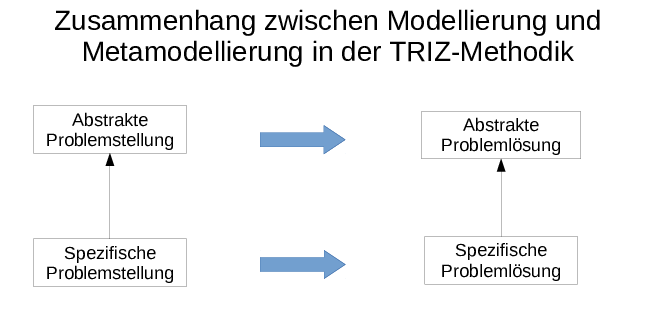
\includegraphics[width=.7\textwidth]{2019-04-25/Folie-1.png}
\end{center}
Im Gegensatz zu Altschullers Anfängen stehen mit den TRIZ-Werkzeugen heute
umfangreiche, auf Erfahrungen aufbauende Werkzeuge zur Verfügung, um
Lösungsvorschläge für das allgemeine Problem zu generieren.

Ziel der Analyse der Patentschrift ist es, die Tauglichkeit dieser allgemeinen
Prinzipien auf dem Kontext der in der Patentschrift beschriebenen speziellen
Problemlösung zu demonstrieren.  Dazu müssen zunächst die spezielle
Problemstellung und die spezielle Lösung inhaltlich und terminologisch
hinreichend aussagekräftig extrahiert werden. Auf der Basis ist schließlich
die Zuordnung zu geeigneten allgemeineren TRIZ-Prinzipien vorzunehmen, wobei
der Herausarbeitung eines \emph{Hauptwiderspruchs} in der speziellen
Problemstellung eine Leitfunktion zukommt.

Ein solcher Widerspruch existiert stets nur \emph{relativ zum Stand der
  Technik}, da es ja gerade das Ziel der verschiedenen TRIZ-Prinzipien ist,
derartige Widersprüche aufzulösen und auf diese Weise einen \emph{neuen Stand
  der Technik} zu etablieren, in welchem die Umgehungsstrategien \emph{dieses}
Widerspruchs Allgemeingut geworden sind.  Damit ist es wichtig, den jeweiligen
Stand der Technik, gegen den die weitere Argumentation geführt wird, genau zu
beschreiben.  Der dem Fachmann als bekannt vorausgesetzte „Stand der Technik“
ist stets ein zeitlich relatives Phänomen, TRIZ dagegen lebt von
ideengeschichtlichen Betrachtungen.

In einigen Fällen kann es schwierig sein, einen solchen Hauptwiderspruch zu
finden.  Hier wäre zu untersuchen, ob es sich bei der patentierten Lösung um
eine \emph{Standardlösung} durch eine nicht offensichtliche
Parameteroptimierung handelt.  Dies ist oft ein Hinweis darauf, dass die
Modellierung des Kontextes zu weit geht und die Auf"|lösung des Widerspruchs
bereits im Stand der Technik subsumiert ist.

Zur Aufbereitung der Patentanalyse sind also die folgenden Schritte
erforderlich:
\begin{itemize}
\item[1.] Erfassung der Metadaten zum Patent.
  
\item[2.] Beschreibung des Stands der Technik in Bezug auf die
  Problemstellung.

  Ein Patent muss grundsätzlich eine \emph{Erfindungshöhe} gegenüber dem Stand
  der Technik aufweisen, das heißt eine für den Fachmann nicht naheliegende
  Lösung beschreiben.  Die zu beschreibende Patentlösung wird nur in einem
  solchen \emph{Kontext} bisheriger technischer Entwicklungen verständlich,
  die einem Fachmann bekannt sind, nicht aber dem Leser der Seminararbeit.
  Dieser ideengeschichtliche Kontext (der auch für die TRIZ-Analyse wichtig
  ist) muss deshalb zunächst \emph{hinreichend genau} beschrieben werden.

\item[3.] Beschreibung des funktionalen Modells.

  Nach der Markierung dieses Kontextes ist es erforderlich, die
  Begriff"|lichkeiten genauer darzustellen, welche für die mit dem Patent
  gelöste Problemstellung erforderlich sind. 

  Dazu sollte zunächst das zu betrachtende System innerhalb eines Obersystems
  abgegrenzt werden. Ein solches System erfüllt innerhalb eines Obersystems
  oft eine spezifische Funktion, die an dieser Stelle herauszuarbeiten ist. 
  
  Hierfür kann die \emph{Innovations-Checkliste} [KS: Kap. 5.1] eine gute
  Hilfestellung sein.  Weiterhin kann es dabei sinnvoll sein,
  \begin{itemize}
  \item Funktionen -- Hauptfunktion(en), Nebenfunktionen [KS: Kap. 4.1.],
    sowie 
  \item Ressourcen -- Typ, Eigenschaften, Verhalten [KS: Kap. 4.2]
  \end{itemize}
  innerhalb des Systems zu identifizieren. 

\item[4.] Formulierung des \emph{Miniproblems}: Herausarbeitung des
  grundlegenden Problems als \emph{spezielles Problem} in einer
  Widerspruchsformulierung.

\item[5.] Beschreibung der Lösung des Problems in der Patentschrift als
  \emph{spezielle Problemlösung}.

\item[6.] Einordnung des Problems in die TRIZ-Systematik als \emph{allgemeines
  Problem}. 

\item[7.] Darstellung des Bezugs der speziellen Lösung zu den allgemeinen
  TRIZ-Strukturen. 
\end{itemize}

Die anzuwendende Methodik ist im folgenden Beispiel prototypisch ausgeführt. 

\section{Beispiel: Das Patent EP0066122B1}

\subsection{Metadaten}
\begin{itemize}\itemsep0pt
\item Titel: Differentialgetriebe
\item Quelle: \url{https://patents.google.com/patent/EP0066122B1}
\item Patentinhaber: Theodoros Tsiriggakis
\item Patentdaten: Veröffentlichung 1982-12-08, Bekanntmachung der
  Patenterteilung 1985-05-15
\item Einordnung durch Google:
  \begin{itemize}
  \item F16 H 48/147 Differentialgetriebe ohne Zahnräder mit Umlaufbewegung
    mit Nocken mit angetriebenen Nockenstößeln oder Kugeln, die in zwei
    gegenüberliegende Nocken eingreifen
  \end{itemize}
\end{itemize}

\subsection{Beschreibung des Stands der Technik}

Wenn ein Fahrzeug durch eine Kurve fährt, legen die äußeren Räder einen
weiteren Weg zurück als die inneren und müssen sich daher schneller drehen.
Dazu muss die Rotationsgeschwindigkeit der Antriebsachse mit
unterschiedlichen, der jeweiligen Fahrsituation angepassten
Übersetzungsverhältnissen auf die angetriebenen Wellen der Laufräder
übertragen werden.

Dies geschieht üblicherweise mit einem Differentialgetriebe auf der Basis von
Zahnrädern. Dazu werden auf die beiden angetriebenen Wellen, die auf einer
gemeinsamen Achse sitzen, Zahnkränze montiert und durch ein oder mehrere
Ritzel miteinander verbunden.  Diese Ritzel vermitteln die
Differenzgeschwindigkeit zwischen beiden Wellen.  Die Antriebsenergie kann
direkt auf eine der beiden Wellen geleitet oder über ein Kronrad auf
verschiedenen Wegen in die Getriebekonstruktion eingebracht werden, etwa --
vergleichbar zu dieser Patentschrift -- indem die Ritzel fest mit dem Kronrad
verbunden sind.  In diesem Fall wird über die Ritzel nicht nur der
Geschwindigkeitsausgleich vermittelt, sondern auch die Kraftübertragung. 
Genauere Ausführungen dazu sind in der Wikipedia [DG] zu finden.

In der Klasse F16H48 der [IPC] werden Patente zu verschiedenen Ausführungen
solcher Differentialgetriebe erfasst.  In einer Klasse von
Differentialgetrieben werden statt eines Ritzels Wälzkörper verwendet, um den
Geschwindigkeitsausgleich zwischen zwei Tellern zu besorgen, die auf den
angetriebenen Wellen montiert sind.  Dieses Prinzip wurde 1932 von Andrew
Francis Ford patentiert (Patent US1897555) und wird in der vorliegenden
Patentschrift als „gattungsbildender Stand der Technik“ bezeichnet, der auch
als Patentklasse F16H48/147 in der [IPC] verzeichnet ist.  Es kann also davon
ausgegangen werden, dass auch zum Zeitpunkt der Einreichung der Patentschrift
diese grundsätzliche Art der Ausführung eines Differentialgetriebes zum „Stand
der Technik“ gehörte.

Als bisherige Probleme sind vor allem Reibungsverluste der Wälzkörper
aufgeführt, die zu unruhigem Lauf und schnellem Verschleiß führen.  Außerdem
kann bei konventioneller Ausfüh\-rung eines Differentialgetriebes auf Glatteis
ein Rad mit doppelter Geschwindigkeit durchdrehen, während das andere
stillsteht.

\subsection{Funktionales Modell}

\paragraph{Obersystem:}
Eintrag von Rotationsenergie über die Antriebswelle, Übertragung der
Rotationsenergie auf die beiden angetriebenen Wellen unter Anpassung der
Geschwindigkeit, um die Laufräder entsprechend anzutreiben. 

\paragraph{Komponenten:}
\begin{itemize}
\item \emph{Angetriebene Wellen} -- mit den Laufrädern verbundene Wellen, die
  auf einer gemeinsamen Achse, der \emph{Systemachse}, montiert sind. 
\item \emph{Kraftübertragungselement}, \emph{Umlaufradträger} (auch Käfig oder
  Korb) -- Eintrag der Antriebsenergie in das System über die antreibende
  Welle, relativ zu welcher die Geschwindigkeiten der beiden angetriebenen
  Wellen adjustiert werden müssen.  In der Patentschrift als \emph{Kronenrad}
  ausgeführt, das parallel zu den Nockenbahntellern liegt, so dass eine feste
  Verbindung zwischen Kronenrad und Nockenbahntellern eine gleichmäßige
  Drehbewegung auf die angetriebenen Achsen leiten würde.
\item \emph{Nockenbahn} -- konzentrisch zur Achse des Nockenbahntellers
  ausgeführte Führungs\-struktur für die Wälzkörper auf dem Nockenbahnteller,
  über welche die Bewegung der Wälzkörper gesteuert wird.  Ein Wälzkörper
  liegt auf den entsprechenden Nockenbahnen der gegenüberliegenden
  Nockenbahnteller auf und dreht sich mit der Differenzgeschwindigkeit der
  angetriebenen Räder.
\item \emph{Nockenbahnteller} -- Übertragungseinheit der Bewegung auf eine der
  angetriebenen Wellen. Mit einer Keilwellenverzahnung wird erreicht, dass
  sich die Nockenbahnteller in Richtung der Systemachse verschieben können.
  Die dabei erforderliche Rück\-stell\-kraft durch eine Feder, welche die
  Nockenbahnteller an die Wälzkörper presst, ist nicht aufgeführt und gehört
  wohl zum Stand der Technik.
\item \emph{Systemachse} -- gemeinsame Drehachse der Nockenbahnteller und des
  Kronenrads. 
\item \emph{Wälzkörper} -- in dieser Patentschrift komplex ausgeführtes
  Übertragungselement zur Drehzahlanpassung und gleichzeitigen
  Kraftübertragung vom Kronenrad auf die Nockenbahnteller und weiter auf jede
  der beiden angetriebenen Wellen.
\end{itemize}

\paragraph{Arbeitsweise des Systems:}
Von der Antriebswelle wird die Rotation starr auf das Kronenrad und weiter auf
die im Kronenrad fixierte Wälzkörperstruktur übertragen, welche die
Drehbewegung über die Nockenstrukturen auf die beiden Nockenbahnteller
übertragen und durch entsprechende Eigendrehbewegungen zugleich für den
Geschwindigkeitsausgleich entsprechend der über die angetriebenen Wellen
eingetragenen Geschwindigkeitsdifferenzen sorgen.

Die Wälzkörper sind in „Käfigstrukturen“ so auf dem Kronenrad fixiert, dass
sie sich mit dem Kronenrad mitbewegen und sowohl die Kraftübertra\-gung als
auch den Geschwindigkeitsausgleich zu den Nockenbahntellern nur durch
eingeschränkte Bewegungen relativ zum Kronenrad vermitteln können.  Die
Wälzkörper können sich dabei senkrecht zur Drehrichtung des Kronenrads bewegen
sowie um die eigene Achse drehen.
  
\subsection{Formulierung des Miniproblems}

Für guten Grip (Kraftübertragung) müssen die Wälzkörper möglichst fest mit den
Nockenbahntellern verbunden sein, für den Ausgleich der Geschwindigkeiten
müssen sie frei auf den Nockenbahnen abrollen.

Die Wälzkörper sollen sich also (zum Geschwindigkeitsausgleich) drehen und
(zur Kraftüber\-tragung) zugleich nicht drehen. 

Bei der Ritzellösung steht das Drehen im Vordergrund, weshalb es unter
extremen Betriebsbedingungen zum Durchdrehen eine Rads bei gleichzeitigem
Stillstand des anderen Rads kommen kann. 

\subsection{Beschreibung der Lösung des Problems in der Patentschrift}

Durch eine sinusförmige Ausführung der Nockenbahnen -- in den Minima ist der
Grip besonders hoch, da hier die potenzielle Energie minimiert wird, in den
Maxima ist die Rollbewegung besonders günstig, da hier kein
Potenzialwiderstand zu überwinden ist -- wechseln Lagen mit hoher
Kraftübertragung und Lagen mit geringem Rollwiderstand.

Durch die Ausführung von zwei Nockenbahnen, die gegeneinander verdreht sind,
wird erreicht, dass die Wälzkörper auf einer Bahn im Minimum sind und damit
maximalen Grip vermitteln, wenn die Wälzkörper auf der anderen Bahn das
Maximum durchlaufen.

Wälzkörper führen sowohl Geradeausbewegungen (senkrecht zur Rotationsebene,
entsprechend dem Stand auf der Nockenbahn) als auch Drehbewegungen aus.  Die
vertikalen Verschiebungsbewegungen werden durch die beiden Nockenbahnen
phasenversetzt getriggert, die Drehbewegungen durch das von den angetriebenen
Achsen übermittelte Geschwindigkeitsdifferential.  Beide Bewegungen zeigen
unterschiedliches Reibungsverhalten.  Durch einen Schichtenaufbau der
Wälzkörper wird erreicht, dass in der ersten Schicht die „Geradführung“ längs
der Systemachse in einer V-förmigen Nut und in der zweiten Schicht die
„Drehlagerung“ in einer kegelförmigen Aussparung ausgeführt ist.  Die
Gesamtbewegung wird also in diese zwei Bewegungen separiert, um die für die
jeweilige Bewegung vorteilhafteste konstruktive Form zu realisieren.

Die Nockenbahnteller sind symmetrisch zueinander ausgeführt, was eine
besonders einfache Herstellung ermöglicht.

Die Nockenbahnteller übertragen in der Grundstellung das gleiche Moment auf
die Achsen und rutschen bei einer Differenz der Drehzahlen immer wieder in
diese Grundstellung, so dass der oben beschriebene „Glatteiseffekt“ nicht
auftreten kann.

\subsection{Einordnung des Problems in die TRIZ-Systematik}

Die Lösung lässt sich nicht direkt in die \emph{Widerspruchsmatrix nach
  Altschuller} einordnen, da hier die Kraftübertragung und der Rollwiderstand
in einem Konflikt zueinander stehen.

In der \emph{Widerspruchsmatrix 2003} lässt sich das Problem nur grob als
Konflikt zwischen Kraft und Geschwindigkeit einordnen, von den  vier
Vorschlägen ist nur das Prinzip der Dynamisierung umgesetzt.

Die Lösung hat insgesamt eher den Charakter einer weiter optimierten, im
Prinzip bereits gefundenen Lösung (Gestaltung der Nockenbahn, genauer Aufbau
der Wälzkörper).

\subsection{Darstellung des Bezugs der speziellen Lösung zu den
  TRIZ-Strukturen} 

Die Lösung erfolgt durch Dynamisierung sowie räumliche Separation sowohl auf
der Nockenbahn als auch im Aufbau der Wälzkörper.

Durch die sinusförmige Ausführung (odp:P19, Prinzip der periodischen Wirkung)
wechseln Bereiche mit guten Grip (Minima) der Wälz\-körper mit Bereichen mit
besserer Rolleigenschaft (odp:P15, Prinzip der Dynamisierung).

Durch die Aufteilung der Wälzkörper wird deren komplexe Bewegung in eine
lineare und eine Drehbewegung separiert, um für beide getrennt jeweils
optimale konstruktive Lösungen zu ermöglichen (odp:P01, Prinzip der
Zerlegung).

Durch die Aufteilung in zwei um $45^\circ$ versetzte Nockenbahnen (odp:P01,
Prinzip der Zerlegung) wird überdies erreicht, dass Wälzkörper stets im
Bereich mit gutem Grip sind und so eine ausreichende Kraftübertragung auf
\emph{beide} angetriebenen Wellen stets gewährleistet ist.

Bereits im Stand der Technik integriert ist die Konzentration von zwei
Funktionen (Drehzahlausgleich und Kraftübertragung) in den Wälzkörpern
(odp:P06, Prinzip der Universalität), die Käfigstruktur, über die Kronenrad
und Wälzkörper miteinander verbunden sind (odp:P07, Prinzip der
Verschachtelung), sowie die rotationssymmetrische Ausführung der Wälzkörper
(odp:P14, Prinzip der Kugelähnlichkeit) sowie überhaupt die Verwendung von
Wälzkörpern (odp:P24, Prinzip des Vermittlers).

\section{Literatur}
\raggedright
\begin{itemize}
\item {[DG]} Wikipedia-Eintrag „Differentialgetriebe“.
  \url{https://de.wikipedia.org/wiki/Differentialgetriebe} (20.07.2019).
\item {[IPC]} International Patent Classification.
  \url{https://www.wipo.int/classifications/ipc/ipcpub} (20.07.2019).
\item{[KS]} Karl Koltze, Valeri Souchkov: Systematische Innovation. 2.,
  überarbeitete Auf"|lage. Hanser Verlag, München 2017.
\item{[PS]} Patentschrift EP0066122B1, veröffentlicht am 15.05.1985 durch das
  Europäische Patentamt. 
\item{[ZH]} Dietmar Zobel, Rainer Hartmann: Erfindungsmuster. 2.,
  durchgesehene Auf"|lage. Expert Verlag, Renningen 2016.
\end{itemize}

   
\vfill
\ccnotice
\end{document}
